\chapter{Design}
\label{design}

This chapter sets out to describe the approach taken to designing a software solution for the requirements discussed in the previous chapter.  It outlines the key concepts behind the user interface design, after which it discusses the different approaches taken in structuring the classes used to model the problem, before going on to describe the database tables that are used.

The chapter begins with a description and depiction of the architecture used, before going on to discuss the rest of the design with the requirements and lessons learned from background research in mind. 

\section{System Architecture}
Non-functional requirement 1 states that interaction with the system should take place through a web-based interface.  This requirement fits well with the client-server model: a set of clients that call on the services offered by a server (or set of servers), facilitated by a network \cite{sommerville}.  The approach taken by the solution is illustrated by the \gls{aod} in Figure \ref{fig:aod}, which is intended to bring the system to life for a reader.

This architecture could, with some reconfiguration, be scaled up to run on multiple servers, including the possibility of separating the database onto another machine, as well as replicating the application across different load-balanced systems.  It was sufficient for deployment of the project to centralise all of the functionality to one piece of hardware, and a \gls{vm} was produced so that it could be emulated on other hardware.

\begin{figure}
	\begin{center}
		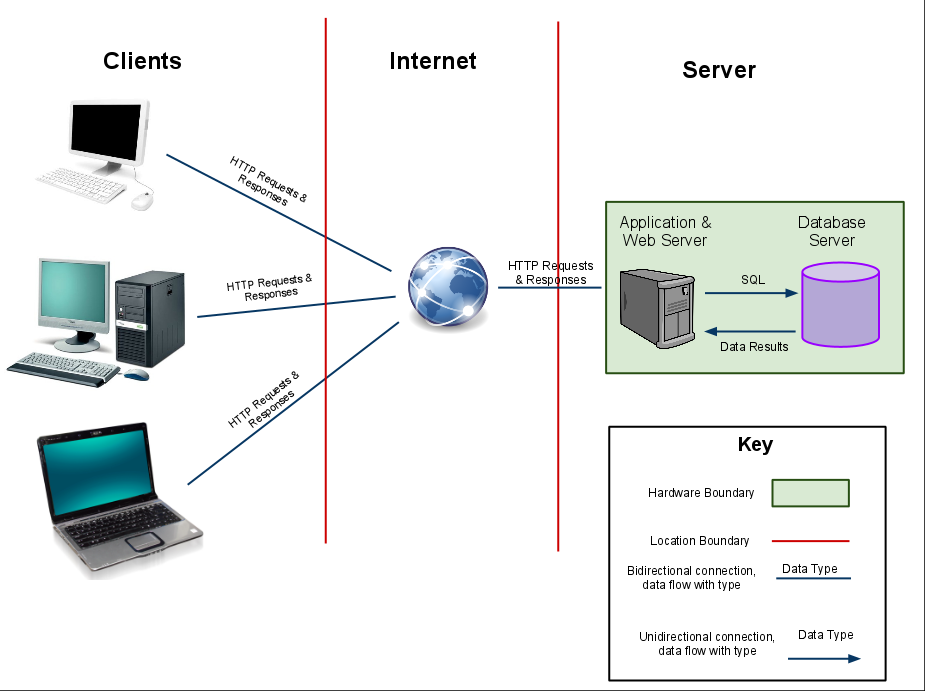
\includegraphics
			[scale=0.45]
			{images/ArchitectureOverviewDiagram.png}
		\caption{High Level Architecture Overview Diagram}
		\label{fig:aod}
	\end{center}
\end{figure}

\begin{figure}
	\begin{center}
		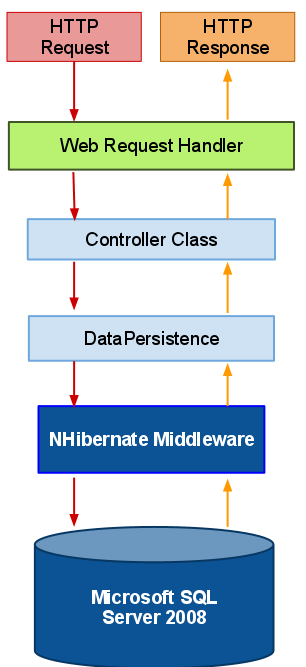
\includegraphics
			[scale=0.45]
			{images/DataFlow.png}
		\caption{Diagram showing high-level data flow between components}
		\label{fig:dataFlow}
	\end{center}
\end{figure}

\section{Web Interface Design}
\label{uiDesign}
The interface design was conceptualised around the idea of a clean, consistent and intuitive interface, in line with the requirements and background findings.  It was important to take account of Fitts' Law, the observation that the smaller a target is, the harder it is for a human to point at and act upon accurately \cite{fitts} (particularly in the 2-dimensional space of a screen \cite{fitts2d}), and to adopt a common sense approach when deciding how large or small clickable items should be.

\section{Class Designs}
This section discusses the class designs as they evolved over different versions of the program, as well as reasons for changes.  Each version is named after NASA Space Shuttle orbiters in chronological order of when they entered service.

An \gls{oo} approach was taken with the project, as the entries that were to be saved mapped well to the concept of an object, and because the \cs{} language is a natively \gls{oo} language.  The \cs{} language is discussed in more detail in Section \ref{csharpDiscussion}.


\begin{figure}
	\begin{center}
		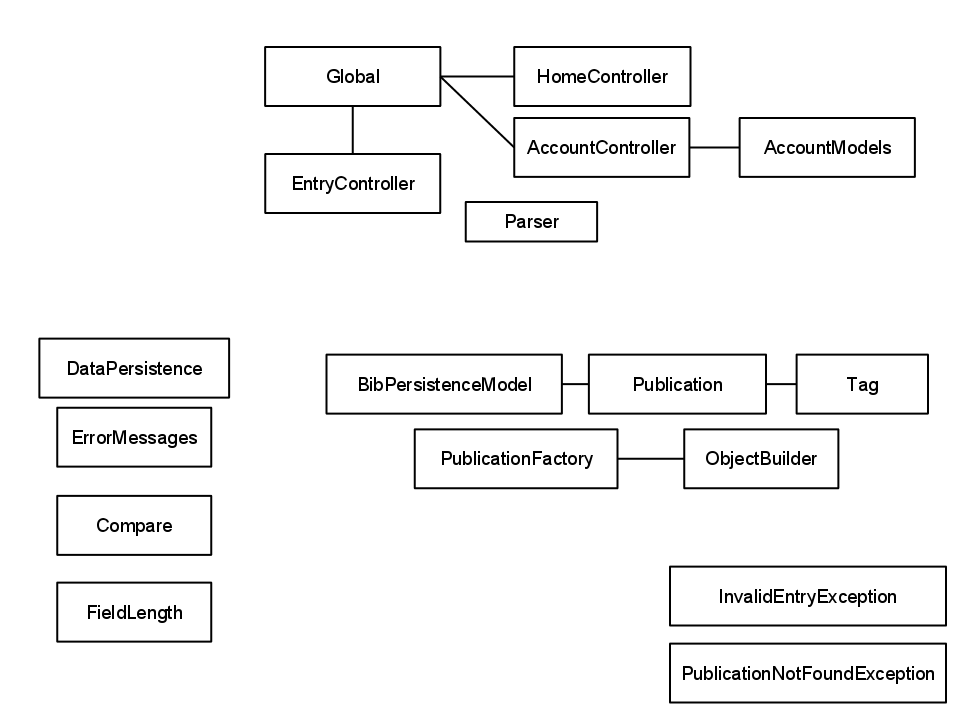
\includegraphics
			[scale=0.45]
			{images/OverallClassDiagram.png}
		\caption{UML Class Diagram showing all classes}
		\label{fig:OverallClassDiagram}
	\end{center}
\end{figure}


% reset mvc acronym.
\glsreset{mvc}
\subsection{Model View Controller}
The application's design is heavily based on the \gls{mvc} architecture.  The data model and database interaction are all taken care of in core classes, namely the \texttt{DataPersistence} and \texttt{Publication} classes.

\subsection{First model version (V0.34 - Columbia)}
\label{columbia}
The approach of the first model version was heavily based on the approach of Mitesh Furia; it was seen as advantageous to reuse the code from his project as much as possible, to reduce development effort and increase the output functionality at the end of this project.  With this aim in mind, the class design for the initial model was heavily structured around his approach.  This approach did not survive the entirety of the project; as development progressed, it became apparent that the design would need to be refactored and streamlined, as discussed in Section \ref{designChallenger}.  The main surviving item from Mitesh's solution was the file parser, which was modified to suit the \cs{} language (from Java) and to provide further feedback to users.

The initial class design consisted of one class per entry type (see Figure \ref{fig:ColumbiaClassDesign} --- an example list of which fields are required and which are optional are shown in Figure \ref{fig:ArticleFields}).  The main focus behind this approach, aside from following Mitesh's successful approach, was to take advantage of a feature of the \gls{net} Framework called Attributes, which can be used effectively for validation.  Attributes provide the ability to associate extra information with each member variable of a class; as an example, the `required' attribute can be used to enforce the requirement to include data in a field for it to be valid.  This approach worked well for this version of the model, boasting excellent robustness to poor or erroneous user input as well as excellent feedback to users through the provision of error messages assigned by the required attribute.  Optional fields were included as member variables, and took advantage of the `DisplayName' attribute. The \gls{net} framework allows automatic generation of labels for web pages, so when a member name doesn't have spaces it results in poor display on the interface.  An example of a member variable name lacking spaces is the field `howpublished': it is more readable and therefore more user friendly when the field is displayed as `how published', which is achieved as shown in Figure \ref{fig:displayName}.

\begin{figure}
	\begin{center}
			\lstset{language=CSharp} 
			\begin{lstlisting}
  // The attribute
  [DisplayName("Book Title")]
  // The member name with no spaces
  public virtual string Booktitle { get; set; }
			\end{lstlisting}
		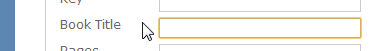
\includegraphics{images/displayNameOnInterface.png}
		\caption{Use of a field name attribute to display a field name differently}
		\label{fig:displayName}
	\end{center}
\end{figure}

\begin{figure}
	\begin{center}
		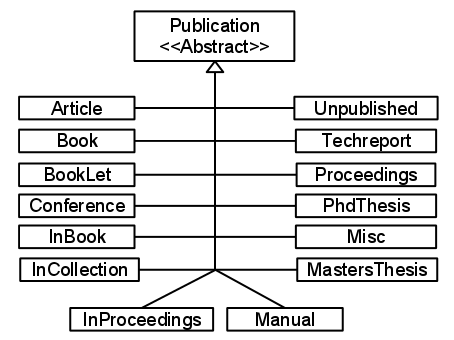
\includegraphics
			[scale=0.6]
			{images/ColumbiaClassDiagram.png}
		\caption{UML Class Diagram of the Columbia Model}
		\label{fig:ColumbiaClassDesign}
	\end{center}
\end{figure}

\begin{figure}
	\begin{center}
		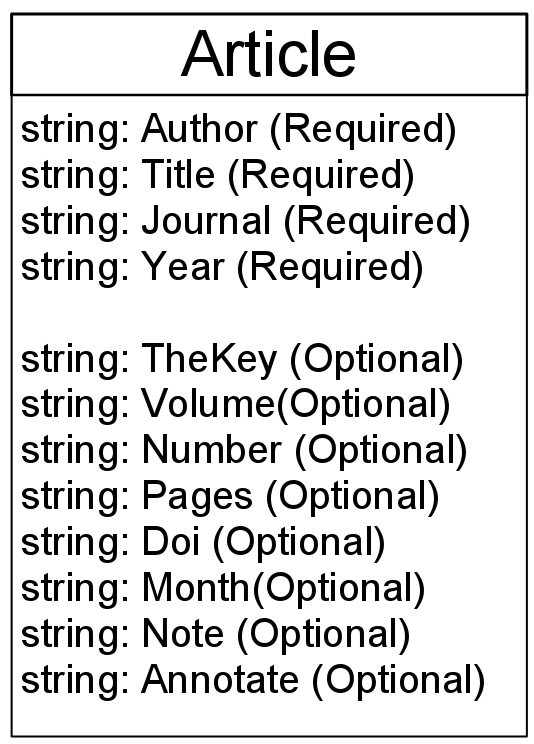
\includegraphics
			[scale=0.3]
			{images/ArticleFields.png}
		\caption{UML Class Diagram showing the required and optional fields for the `Article' entry type}
		\label{fig:ArticleFields}
	\end{center}
\end{figure}

Each entry type was a subclass of the abstract superclass \texttt{Publication}, which contained fields common to all entry types, namely: Id, an int identifier; CiteKey, a string intended to be unique to an entry, but not usable as an identifier in the database, allowing duplicate entries to exist in the system; Owner, the username of the user who created the entry in the first instance; along with Abstract, a string field which was to be optional to all entries.

As the class was designated `abstract', the enforcement of rules associated with the concept\footnote{Designating a class `abstract' means that an instance of it cannot be directly created, but an inheriting concrete (antonym of abstract) can be instantiated.} were used to the advantage of the developer: several methods, which were to be relied on and required by the controller classes, were added as abstract methods to the Publication class.  These abstract methods included two methods which converted an entry to a string representing the entry as a row in a \gls{html} table, both with and without hyperlinks to the amendment page for the entry.


\subsection{Second model: V1.0 - Challenger}
\label{designChallenger}
The Challenger model was the model adopted in the final (deployed) version of the product.  This is the model that is discussed during the implementation chapter (Chapter~\ref{impl}).

Columbia's design presented a few problems for development and performance on the system, as was discovered after implementation:
\begin{enumerate}
	\item 14 entry types meant 14 tables and 14 queries to search for an entry or retrieve all entries, which had a serious impact on performance;
	\item Identifiers were unique to each table only, and did not necessarily identify an entry from all others, which resulted in problems with access by the application.
\end{enumerate}

To solve these problems, a large refactoring took place to reposition all entries' fields in the top-level class \texttt{Publication}.  This reduced the class diagram for the model from as shown in Figure \ref{fig:ColumbiaClassDesign} to as shown in Figure \ref{fig:ChallengerClassDiagram}

\begin{figure}
	\begin{center}
		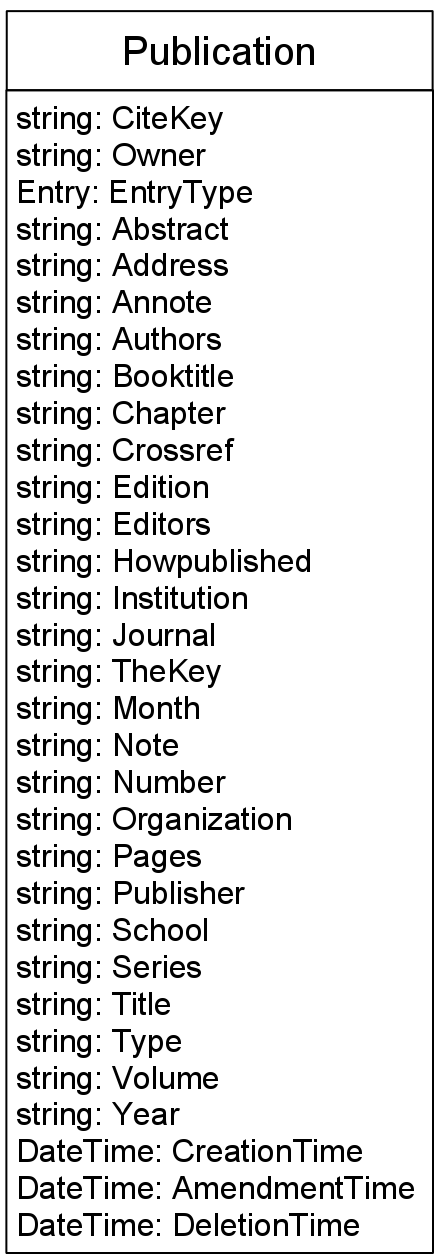
\includegraphics
			[scale=0.3]
			{images/ChallengerClassDiagram.png}
		\caption{UML Class Diagram of the Challenger Model}
		\label{fig:ChallengerClassDiagram}
	\end{center}
\end{figure}

This directly maps to the database model

Single table for all entry types:\\
why\\
what improved?\\
 - faster search\\
 - IDs all in one place - less complicated - don't need to kow what an entry's type is before searching it\\

\subsection{Third (proposed) model: V2.0 - Discovery}
\label{designDiscovery}
Discovery was intended to add a feature called `tagging' to the system.  \\
Specifically, this was to involve a many-to-many mapping from \texttt{Publication} to \texttt{Tag}


\section{DB Design Diagram}
content
